\documentclass[11pt]{article}
\usepackage[margin=0.75in]{geometry}
\usepackage{graphicx}
\usepackage{booktabs}
\usepackage{array}
\usepackage[T1]{fontenc}
\title{KUMMER-N13: Concrete 16-bit State Replay}
\author{Source-bound research packet}
\date{25 October 2026}
\begin{document}
\maketitle
\noindent The actual cached theta xADD and signed-recovery source was replayed
on every signed state in three frozen 16-bit odd-prime subgroups. The source
produced three xADD outputs and one signed lift per state. An independent
Jacobian oracle checked the outputs. This is finite exhaustion of these three
groups, not a bound for the other 18 frozen models.

\begin{center}
\begin{tabular}{r r r r r r}
\toprule
$p$ & states & xADD calls & xADD errors & lift correct & lift no divisor\\
\midrule
739 & 34,147 & 102,441 & 0 & 33,856 & 291\\
1,151 & 41,399 & 124,197 & 0 & 41,256 & 143\\
1,187 & 44,027 & 132,081 & 0 & 43,892 & 135\\
\midrule
Total & 119,573 & 358,719 & 0 & 119,004 & 569\\
\bottomrule
\end{tabular}
\end{center}

\noindent The fast signed-recover branch failed on 1,063 states. Its
enumerated fallback recovered 494 of them: 170, 190, and 134 by model.
The final 569 no-divisor states are after this fallback; none are unaccounted
for. The 569 failures
split into 108 \texttt{Delta\_zero}, 108 \texttt{b1\_coefficient\_zero}, and
353 \texttt{general\_conversion\_inapplicable}. These are current
implementation branch failures. They do not contradict the abstract
pair-sign uniqueness theorem.

\noindent The lift calls used 41,887,801 M, 33,639,052 A, and 2,268,451 I
in signed recovery after cached inverse setup. Exceptional enumeration added
92,925 field M, 1,482 field S, 3,677 field I, 169,982 field additions, and
741 Jacobian additions. These counters exclude setup, labels, collector work,
relation processing, and end-to-end checks. No ratio to rho is measured.

\noindent Evidence: \texttt{results/states.csv} (one row per scalar),
\texttt{results/summary.json} (source and CSV digests), and
\texttt{SHA256SUMS}. Native \texttt{validate} recomputes counts and digests.
The 18 larger models, all-state fallback proof, full target cohort, and
matched rho pricing remain open.

\begin{center}
\centering
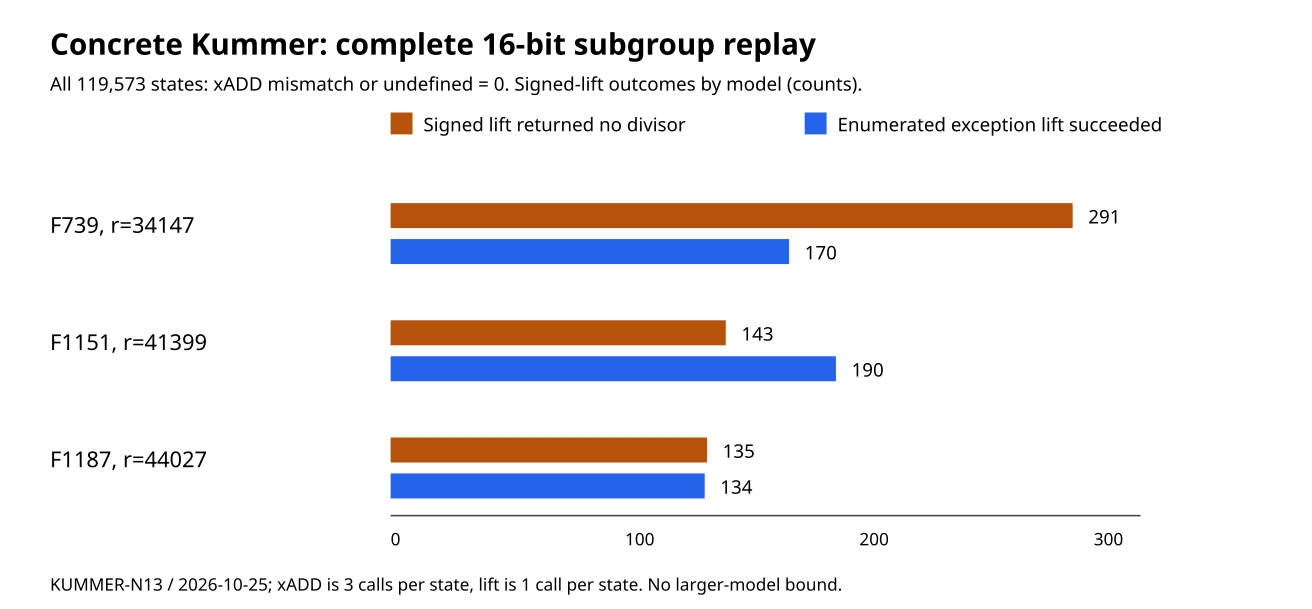
\includegraphics[width=0.74\linewidth]{research/kummer_differential_collector_20261022/n13-concrete-gate/status-graph.png}\\
\small Counts from the 119,573 per-state records; KUMMER-N13, 2026-10-25.
\end{center}

\end{document}
